\subsection{Stakeholders}
Industry Sponsor : Portland State University Electrical and Computer Engineering Dept, WEST Lab (Dr. David C. Burnett) \\
Faculty Advisor: Dr. John M. Acken\\
Engineers: \begin{itemize}
\item Adam A. Dezay
\item Manuel A. Garcia
\item Brandon P. Hippe
\item Mercedes C. Newton \\
\end{itemize}
Customer: Any business or person in need of monitoring changing air quality conditions.

\subsection{Pre-existing Design}
This project used some of the research done in last year’s capstone project. The final report from last year’s project can be found under the documentation folder in the team’s Github repository. The file is titled \texttt{Team 13 -- Final Report -- SensorSuite.pdf}. Link to the Github can be found in the project resources section.\\
\\
\begin{figure}[H]
    \centering
    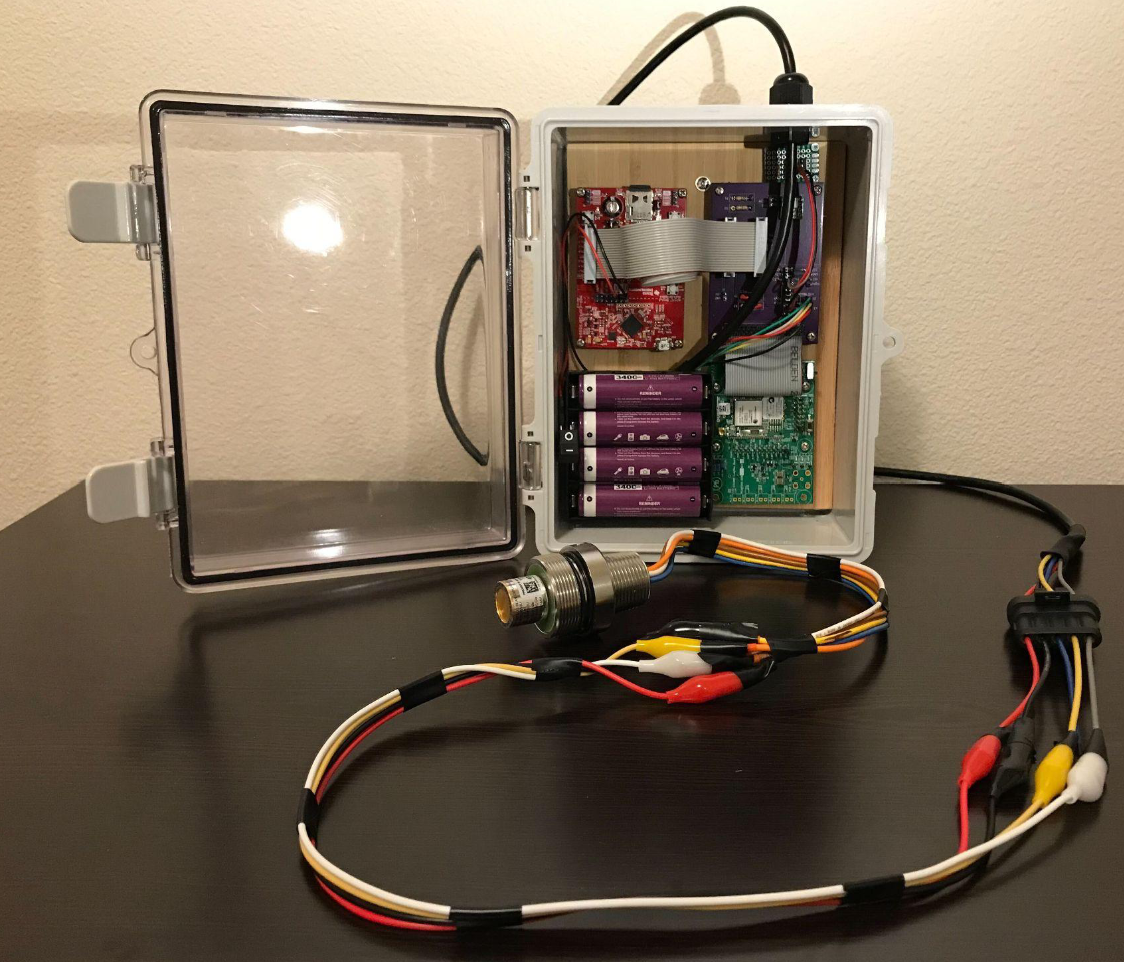
\includegraphics[width=0.8\textwidth]{Pictures/prevproj.png}
    \caption[Previous Teams Project]{Previous Teams Project} 
    \cite{leon2023networked}
    \label{fig:part1commrin}
\end{figure}
Even though last year’s project measured temperature, humidity, and N$_2$O outdoors, both projects share the same controller, the MSP430. They both also use SmartMesh IP as a way to connect multiple nodes. \\
\\
We faced many challenges with the microcontroller as well as SmartMesh that last year’s team did not experience. Check Appendix A to see the solutions to unexpected problems we encountered that the previous team did not. 